\section{Техническое задание}
\subsection{Основание для разработки}

Основанием для разработки является потребность в создании веб-мессенджера в рамках проекта по предмету "Проектирование и разработка программных систем".

\subsection{Цель и назначение разработки}

Основной целью данного проекта является разработка веб-мессенджера с использованием технологий Python для серверной части, а также JavaScript, HTML и CSS для клиентской части.

Целью разработки веб-мессенджера является предоставление эффективного инструмента для обмена мгновенными сообщениями в веб-пространстве, обеспечивая удобство использования и современные функциональные возможности.

Задачи данной разработки включают:
\begin{itemize}
	\item Создание серверной части мессенджера на языке Python, обеспечивающей обработку сообщений, управление пользователями и хранение данных.
	\item Разработка клиентской части веб-мессенджера, используя JavaScript, HTML и CSS для обеспечения удобного пользовательского интерфейса.
	\item Реализация механизмов обмена сообщениями в режиме реального времени.
	\item Обеспечение безопасности обмена данными и внедрение технологий шифрования для защиты конфиденциальности.
	\item Тестирование и отладка системы для выявления и устранения возможных ошибок и недоразумений.
\end{itemize}

\subsection{Описание веб-мессенджера}

Веб-мессенджер представляет собой платформу для обмена мгновенными сообщениями между пользователями. Он обладает следующими особенностями:

\begin{enumerate}
	\item \textbf{Многоплатформенность:} Поддержка различных платформ, включая веб-версию, мобильные приложения и настольные приложения.
	\item \textbf{Безопасность и шифрование:} Внедрение технологий шифрования для обеспечения безопасности обмена сообщениями и конфиденциальности данных пользователей.
	\item \textbf{Интеграция с другими сервисами:} Возможность интеграции с другими сервисами и приложениями для расширения функциональности мессенджера.
	\item \textbf{Групповые чаты и коллективная работа:} Поддержка групповых чатов и инструментов для коллективной работы и обмена файлами.
	\item \textbf{Использование искусственного интеллекта:} Возможное использование искусственного интеллекта для улучшения пользовательского опыта и предоставления персонализированных рекомендаций.

\subsubsection{Иконки и элементы интерфейса}
Сообщение - основной элемент взаимодействия пользователей в чате. Отображает текстовое сообщение и информацию об отправителе.
\begin{figure}[H]
	\centering
	
\includegraphics[width=0.7\linewidth]{images/message}
	\caption{Сообщение}
	\label{fig:message}
\end{figure}
Пользователь онлайн - индикатор онлайна пользователя. Отображает, что пользователь в данный момент находится в сети.
\begin{figure}[H]
	\centering
	
\includegraphics[width=0.7\linewidth]{images/online}
	\caption{Пользователь онлайн}
	\label{fig:online}
\end{figure}
"Смайлик"  - иконка, указывающая на отправку "смайликов" в сообщении. Позволяет пользователям отправлять "смайлики".
\begin{figure}[H]
	\centering
	
\includegraphics[width=0.7\linewidth]{images/smile}
	\caption{Кнопка отправки смайликов}
	\label{fig:smile}
\end{figure}

\subsubsection{Функциональные элементы}
Интерфейс должен предоставлять следующие элементы и функции:
\begin{itemize}
	\item Возможность отправки текстовых сообщений.
	\item Возможность прикрепления и отправки файлов.
	\item Отображение онлайн статуса пользователей.
	\item Возможность создания и управления групповыми чатами.
	\item Индикация новых сообщений и уведомлений.
\end{itemize}

Композиция интерфейса мессенджера представлена на рисунке ~\ref{fig:maket2}.

\begin{figure}[H]
	\centering
	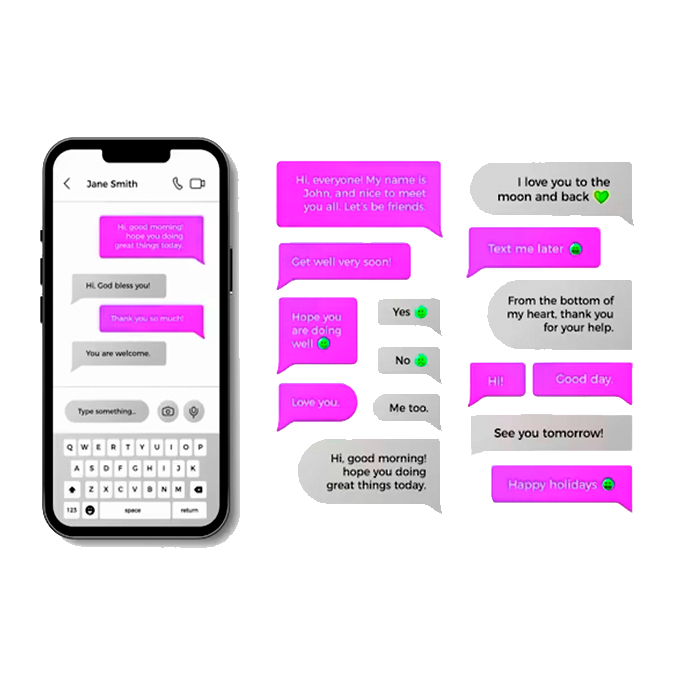
\includegraphics[width=0.7\linewidth]{images/komp_messenger}
	\caption{Композиция мессенджера}
	\label{fig:kompmessenger}
\end{figure}

\subsection{Требования пользователя к интерфейсу веб-мессенджера}

Веб-мессенджер должен обеспечивать удобное взаимодействие пользователей и предоставлять следующие возможности:
\begin{itemize}
	\item Отправка текстовых сообщений: Пользователи должны иметь возможность обмениваться текстовыми сообщениями для эффективного общения.
	\item Отправка смайликов: Возможность отправлять смайлики, обеспечивая обмен различными эмоциями.
	\item Полная авторизация для дальнейшего отображения имени в чате.
\end{itemize}

%\begin{figure}[ht]
%\caption{Композиция шаблона сайта}
%\label{templ:image}
%\end{figure}
%\vspace{-\figureaboveskip} % двойной отступ не нужен (можно использовать, если раздел заканчивается картинкой)

\subsection{Моделирование вариантов использования}
 \subsubsection{Диаграмма прецедентов}
Для разрабатываемого веб-мессенджера была реализована модель, которая обеспечивает наглядное представление вариантов использования мессенджера.

Она помогает в физической разработке и детальном анализе взаимосвязей объектов. При построении диаграммы вариантов использования применяется унифицированный язык визуального моделирования UML.

На основании анализа предметной области в программе должны быть реализованы следующие прецеденты:
\begin{enumerate}
	\item Регистрация нового пользователя.
	\item Авторизация пользователя.
	\item Отправка текстового сообщения.
	\item Прикрепление и отправка смайликов.
\end{enumerate}

\begin{figure}[ht]
	\center{\includegraphics[width=1\linewidth]{precend}}
	\caption{Диаграмма прецедентов}
	\label{precend:image}
\end{figure}

 \subsubsection{Сценарии прецедентов программы}
 
 \begin{enumerate}
 	\item Сценарий для прецедента «Регистрация нового пользователя»:
 	\begin{itemize}
 		\item основной исполнитель: пользователь;
 		\item заинтересованные лица и их требования: пользователю необходимо предоставить уникальный логин и пароль;
 		\item предусловие: пользователь открыл веб-мессенджер в браузере;
 		\item основной успешный сценарий: пользователь вводит уникальный логин и пароль, система регистрирует нового пользователя.
 	\end{itemize}
	\item Сценарий для прецедента «Авторизация пользователя»:
	\begin{itemize}
		\item основной исполнитель: пользователь;
		\item заинтересованные лица и их требования: пользователю необходимо предоставить зарегистрированный логин и пароль;
		\item предусловие: пользователь открыл веб-мессенджер в браузере;
		\item основной успешный сценарий: пользователь вводит зарегистрированный логин и пароль, система производит авторизацию.
	\end{itemize}
	
	\item Сценарий для прецедента «Отправка текстового сообщения»:
	\begin{itemize}
		\item основной исполнитель: пользователь;
		\item заинтересованные лица и их требования: пользователю необходимо написать текст сообщения;
		\item предусловие: пользователь авторизован в системе;
		\item основной успешный сценарий: пользователь вводит текст сообщения, отправляет его.
	\end{itemize}
	
	\item Сценарий для прецедента «Прикрепление и отправка смайликов»:
	\begin{itemize}
		\item основной исполнитель: пользователь;
		\item заинтересованные лица и их требования: пользователю необходимо выбрать смайлик и отправить его;
		\item предусловие: пользователь авторизован в системе;
		\item основной успешный сценарий: пользователь выбирает смайлик, отправляет его.
	\end{itemize}
	
\end{enumerate}

\subsection{Требования к оформлению документации}

Разработка программной документации и программного изделия должна производиться согласно ГОСТ 19.102-77 и ГОСТ 34.601-90. Единая система программной документации.
